\documentclass{standalone}
\input{feynman_settings}

\usetikzlibrary{patterns, decorations.markings, snakes, calc, decorations.pathreplacing, decorations}

\usepackage{relsize} %larger math symbols

\begin{document}

%Setup for the wiggly circle: The idea is to add a sine function to the usual circle 
\tikzset{/pgf/decoration/.cd,
    number of sines/.initial=10,
    angle step/.initial=20,
}
\newdimen\tmpdimen
\pgfdeclaredecoration{complete sines}{initial}
{
    \state{initial}[
        width=+0pt,
        next state=move,
        persistent precomputation={
            \pgfmathparse{\pgfkeysvalueof{/pgf/decoration/angle step}}%
            \let\anglestep=\pgfmathresult%
            \let\currentangle=\pgfmathresult%
            \pgfmathsetlengthmacro{\pointsperanglestep}%
                {(\pgfdecoratedremainingdistance/\pgfkeysvalueof{/pgf/decoration/number of sines})/360*\anglestep}%
        }] {}
    \state{move}[width=+\pointsperanglestep, next state=draw]{
        \pgfpathmoveto{\pgfpointorigin}
    }
    \state{draw}[width=+\pointsperanglestep, switch if less than=1.25*\pointsperanglestep to final, % <- bit of a hack
        persistent postcomputation={
        \pgfmathparse{mod(\currentangle+\anglestep, 360)}%
        \let\currentangle=\pgfmathresult%
    }]{%
        \pgfmathsin{+\currentangle}%
        \tmpdimen=\pgfdecorationsegmentamplitude%
        \tmpdimen=\pgfmathresult\tmpdimen%
        \divide\tmpdimen by2\relax%
        \pgfpathlineto{\pgfqpoint{0pt}{\tmpdimen}}%
    }
    \state{final}{
        \ifdim\pgfdecoratedremainingdistance>0pt\relax
            \pgfpathlineto{\pgfpointdecoratedpathlast}
        \fi
   }
}


%actual code

\hspace{-0.7cm}
\raisebox{4ex}{\Large$\partial_t\Gamma_k[\bar{g}, 0] = \mathlarger{\frac{1}{2}}$
 }

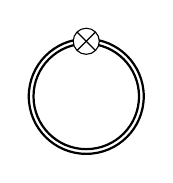
\begin{tikzpicture}[cross/.style={path picture={ 
\draw[black]
(path picture bounding box.south east) -- (path picture bounding box.north west) (path picture bounding box.south west) -- (path picture bounding box.north east);
}}]
\draw[thick] circle(0.73);
\draw[thick] circle(0.67);
\node [draw, fill = white, circle, cross, minimum width= 0.1 cm] at (0,0.7){}; 
\end{tikzpicture}
\raisebox{4ex}{\Large$ \ \ - \ $
 }

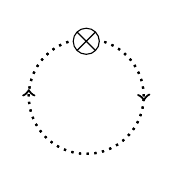
\begin{tikzpicture}[cross/.style={path picture={ 
\draw[black]
(path picture bounding box.south east) -- (path picture bounding box.north west) (path picture bounding box.south west) -- (path picture bounding box.north east);
}}]
\draw[thick, dotted, decoration={markings, mark=at position 0.5 with {\arrow{<}}}, postaction={decorate}] circle(0.73);
\draw[thick, dotted, decoration={markings, mark=at position 0.007 with {\arrow{<}}}, postaction={decorate}] circle(0.73);
\node [draw, fill = white, circle, cross, minimum width= 0.1 cm] at (0,0.7){}; 
\end{tikzpicture}

\raisebox{4ex}{\Large$ \ + \ \mathlarger{\frac{1}{2}}$
 }

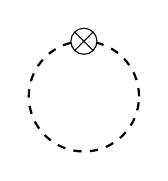
\begin{tikzpicture}[cross/.style={path picture={ 
\draw[black]
(path picture bounding box.south east) -- (path picture bounding box.north west) (path picture bounding box.south west) -- (path picture bounding box.north east);
}}]
\draw[thick, dashed] circle(0.7);
\node [draw, fill = white, circle, cross, minimum width= 0.1 cm] at (0,0.7){}; 
\end{tikzpicture}

\raisebox{4ex}{\Large$ \ \ - \ $
 }

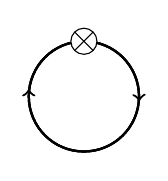
\begin{tikzpicture}[cross/.style={path picture={ 
\draw[black]
(path picture bounding box.south east) -- (path picture bounding box.north west) (path picture bounding box.south west) -- (path picture bounding box.north east);
}}]
\draw[thick, decoration={markings, mark=at position 0.5 with {\arrow{<}}}, postaction={decorate}] circle(0.7);
\draw[thick, decoration={markings, mark=at position 0.007 with {\arrow{<}}}, postaction={decorate}] circle(0.7);
\draw[thick] circle(0.7);
\node [draw, fill = white, circle, cross, minimum width= 0.1 cm] at (0,0.7){}; 
\end{tikzpicture}

\raisebox{4ex}{\Large$ \ + \ \mathlarger{\frac{1}{2}}$
 }
 
 \begin{tikzpicture}[
    sines/.style={
        thick,
        line join=round, 
        draw=black, 
        decorate, 
        decoration={complete sines, number of sines=11, amplitude=4pt}
    },
cross/.style={path picture={ 
\draw[black]
(path picture bounding box.south east) -- (path picture bounding box.north west) (path picture bounding box.south west) -- (path picture bounding box.north east);
}}]

\draw [white, postaction={sines}, thin] 
        (0,0) circle [radius=0.7];
\node [draw, fill = white, circle, cross, minimum width= 0.1 cm] at (0,0.7){}; 

\end{tikzpicture}
\raisebox{4ex}{\Large$ \ \ - \ $
 }

 \begin{tikzpicture}[
    sines/.style={
        thick,
        line join=round, 
        draw=black, 
        decorate, 
        decoration={complete sines, number of sines=11, amplitude=4pt}
    },
cross/.style={path picture={ 
\draw[black]
(path picture bounding box.south east) -- (path picture bounding box.north west) (path picture bounding box.south west) -- (path picture bounding box.north east);
}}]

\draw [densely dotted, white, postaction={sines}, thin] 
        (0,0) circle [radius=0.7];
\node [draw, fill = white, circle, cross, minimum width= 0.1 cm] at (0,0.7){}; 

\end{tikzpicture}
%\raisebox{4ex}{$ \ \ - \ $
%}

%\begin{tikzpicture}[cross/.style={path picture={ 
%\draw[black]
%(path picture bounding box.south east) -- (path picture bounding box.north west) (path picture bounding box.south west) -- (path picture bounding box.north east);
%}}]
%\draw[thick, dotted] circle(0.7);
%\node [draw, fill = white, circle, cross, minimum width= 0.1 cm] at (0,0.7){}; 
%\end{tikzpicture}
\end{document}